\documentclass[12pt]{article}
\usepackage{graphicx}
\usepackage[margin=.5in]{geometry} 
\usepackage{amsmath,amsthm,amssymb}
%\usepackage{gensymb}
  \usepackage{hyperref}
  \usepackage{pdfpages} 
  %\usepackage[table]{xcolor}
  
 %\usepackage{xcolor} % Required for specifying colors by name
\definecolor{ocre}{RGB}{52,177,201} % Define the orange color used for highlighting throughout the book

% Font Settings
\usepackage{avant} % Use the Avantgarde font for headings
%\usepackage{times} % Use the Times font for headings
\usepackage{mathptmx} % Use the Adobe Times Roman as the default text font together with math symbols from the Sym­bol, Chancery and Com­puter Modern fonts

%\usepackage{microtype} % Slightly tweak font spacing for aesthetics
%\usepackage[utf8]{inputenc} % Required for including letters with accents
\usepackage[T1]{fontenc} % Use 8-bit encoding that has 256 glyphs
%\usepackage{soul}
\usepackage{undertilde}
%\usepackage{accents}
\newcommand{\StandardLM}{\by=\bX \bbeta +{\epsilonbf}}

\usepackage{xcolor}
\usepackage{xparse}
\definecolor{lightGray}{gray}{0.95}
\definecolor{lightGrayOne}{gray}{0.9}
\definecolor{lightBlueOne}{RGB}{204, 255, 255}
\definecolor{lightBlueTwo}{RGB}{204, 238, 255}
\definecolor{lightBlueThree}{RGB}{204, 204, 255}
\definecolor{AltBlue}{RGB}{119,14,161}
\definecolor{Orchid}{RGB}{186,85,211}

\definecolor{BGBlue}{RGB}{220,221,252}
\definecolor{BGBlueOne}{RGB}{204,229,255}

\definecolor{DarkGreenOne}{RGB}{34,139,34}

\definecolor{BGGreen}{RGB}{240,243,245}
\definecolor{lightGreenOne}{RGB}{179, 255, 179}
\definecolor{lightGreenTwo}{RGB}{198, 255, 179}
\definecolor{lightGreenThree}{RGB}{243, 255, 230}
\definecolor{AltGreen}{RGB}{193, 240, 240}

\definecolor{BOGreen}{RGB}{180,0,0}
\definecolor{BGGreenOne}{RGB}{220,250,220}

\definecolor{lightBrownOne}{RGB}{255, 221, 204}
\definecolor{lightBrownTwo}{RGB}{255, 229, 204}
\definecolor{lightBrownThree}{RGB}{242, 217, 230}


\definecolor{HLTGreen}{RGB}{230,244,215}
\definecolor{ExcBrown}{RGB}{153,0,0}
\definecolor{ExcBGBrown}{RGB}{255,204,204}
\definecolor{BGYellowOne}{RGB}{255,235,208}
\definecolor{BGPink}{RGB}{255,215,240}

\newcommand{\MakeVec}[1]{{\utilde{\bf #1}}}

\NewDocumentCommand{\MCOption}{O{1.75in} m}{
\TextInBoxTwo[BGPink]{ #1 } {\TextInBoxTwo[white]{.1 in }{ \quad}\HLT{#2}}
}

 \NewDocumentCommand{\ThreeChoices}{O{Do not Know}O{Not confident}O{Confident}}{
\MCOption{#1} \MCOption{#2} \MCOption{#3}
}
 
\NewDocumentCommand{\OneBlock}{ O{HLTGreen} m m }{\colorbox{#1}{\begin{minipage}{#2} $ #3$ \end{minipage}}}

\NewDocumentCommand{\HLT}{ O{HLTGreen} m }{\colorbox{#1}{#2}}
%\NewDocumentCommand{\HLTEQ}{ O{HLTGreen} m }{\colorbox{#1}{$#2$}}
\NewDocumentCommand{\HLTEQ}{ O{white} m }{\colorbox{#1}{$#2$}}

%\newcommand{\HLT}[1]{\colorbox{HLTGreen}{#1}}
\newcommand{\DEHLT}[1]{\colorbox{lightGrayOne}{\color{white} #1}}

\newcommand{\TextInBoxOne}[2]{  {\fcolorbox{white}{lightGrayOne}{\begin{minipage}{#1}  #2 \end{minipage}}}}


\NewDocumentCommand{\TextInBoxTwo}{ O{lightGrayOne} m m } {{\fcolorbox{white}{#1}{\begin{minipage}{#2} { #3} \end{minipage}}}}


\newcommand{\TextInBox}[2]{  {\fcolorbox{BGGreen}{BGGreen}{\begin{minipage}{#1}  #2 \end{minipage}}}}
\newcommand{\TextInBoxCol}[2]{
\fcolorbox{BGBlue}{BGBlue}{%
\begin{minipage}{#1}
 {\color{AltBlue} #2}
\end{minipage}}%
}

\NewDocumentCommand{\TxtBnd}{ O{lightBrownOne} m m } {{\fcolorbox{white}{#1}{\begin{minipage}{#2} { #3} \end{minipage}}}}


\newcommand{\BandInTopBox}[2]{
\fcolorbox{AltBlue}{AltBlue}{%
\begin{minipage}{#1}{ {\color{white}  #2 \hspace{.1in}} }
\end{minipage}}%
}


\newcommand{\TextInBoxThm}[2]{
\fcolorbox{AltBlue}{lightGray}{%
\begin{minipage}{#1}
 {\color{black} #2}
\end{minipage}}%
}

\newcommand{\TextInBoxThmOne}[2]{
\fcolorbox{BGBlue}{BGBlueOne}{%
\begin{minipage}{#1}
 {\color{AltBlue} #2}
\end{minipage}}%
}

\newcommand{\TextInBoxLem}[2]{
\fcolorbox{BGBlue}{lightGray}{%
\begin{minipage}{#1}
 {\color{black} #2}
\end{minipage}}%
}



\newcommand{\TextInBoxLemOne}[2]{
\vspace{.02 in}
\noindent
\fcolorbox{BGBlue}{BGBlue}{%
\begin{minipage}{#1}
 {\color{AltBlue} #2}
\end{minipage}}%
}



\newcommand{\DefBox}[1]{
%\vspace{.1 in}
\noindent
\TextInBoxLem{4.5 in }{
\BandInTopBox{4.4 in }{}
\TextInBoxLemOne{4.4 in }{
#1
}}}





\newcommand{\DefBoxOne}[2]{
%\vspace{.1 in}
\noindent
\TextInBoxLem{4.5 in }{
\BandInTopBox{4.4 in }{#1}
\TextInBoxLemOne{4.4 in }{
#2
}}}


\newcommand{\ThmBox}[2]{
\noindent
\TextInBoxThm{4.4 in }{
\TextInBoxThmOne{4.4 in }{
#1}
#2}
}

\newcommand{\LemBox}[2]{
\noindent
\TextInBoxLem{4.5 in }{
\TextInBoxLemOne{4.4 in }{
#1}
#2}
}

\newcommand{\PropBox}[2]{
\vspace{.1 in}
\noindent
\TextInBoxLem{4.5 in }{
\TextInBoxLemOne{4.4 in }{
#1}
#2}
}




\newcommand{\TextInBoxExc}[2]{
\noindent
\fcolorbox{white}{BGGreenOne}{%
\begin{minipage}{#1}
 {\color{black} #2}
\end{minipage}}%
}


\newcommand{\TextInBoxExample}[2]{
\noindent
\fcolorbox{white}{BGPink}{%
\begin{minipage}{#1}
 {\color{black} #2}
\end{minipage}}%
}


\newcommand{\ExerciseBox}[1]{
\noindent
%\TextInBoxLem{6 in }{
\TextInBoxExc{6 in }{
#1}
%#2}
}


\newcommand{\ExampleBox}[1]{
\noindent
%\TextInBoxLem{6 in }{
\TextInBoxExample{6 in }{
#1}
%#2}
}

\NewDocumentCommand{\CommentBox}{ O{BGBlue}  m }{
\TextInBoxLem{5.5in }{
{\bf Comment:}\\
\TextInBoxLemOne{5.4 in }{
#2}}
}



\newcommand{\HLTY}[1]{\HLTEQ[yellow]{#1}}
\newcommand{\HLTW}[1]{\HLTEQ[white]{#1}}



\newcommand{\qBox}[1]{
  \begin{tikzpicture}
\node[draw=none,shade,
      top color=lightGrayOne,
      bottom color=lightGray,
      rounded corners=2pt,
      blur shadow={shadow blur steps=5}
    ] at (0,0) {    \noindent 
\fcolorbox{white}{BGBlue}{%
\begin{minipage}{4.55 in}
 {\color{black} {
 #1}}
\end{minipage}  }%
 };
 
    \end{tikzpicture}
}
 
 


 

\newcommand{\qBoxCol}[2]{
  \begin{tikzpicture}
\node[draw=none,shade,
      top color=lightGrayOne,
      bottom color=lightGray,
      rounded corners=2pt,
      blur shadow={shadow blur steps=5}
    ] at (0,0) {    \noindent
\fcolorbox{white}{#1}{%
%\begin{minipage}{4.55 in}
\begin{minipage}{4.55 in}
 {
 \color{black} {
 #2}}
\end{minipage}  }%
 };
 
    \end{tikzpicture}
}
  
  
  
  
  
  

\NewDocumentCommand{\qBrd}{O{4.55 in} m m}{
  \begin{tikzpicture}
\node[draw=none,shade,
      top color=#2,
      bottom color=#2,
      rounded corners=2pt,
      blur shadow={shadow blur steps=5}
    ] at (0,0) {    \begin{minipage}{#1}
 {
 \color{black} {
 #3}}
\end{minipage} 

 };
 
    \end{tikzpicture}
}
    
  
  
  
  
\NewDocumentCommand{\qbx}{O{4.55 in} m m}{
  \begin{tikzpicture}
\node[draw=none,shade,
      top color=lightGrayOne,
      bottom color=lightGray,
      rounded corners=2pt,
      blur shadow={shadow blur steps=5}
    ] at (0,0) {    \noindent
\fcolorbox{white}{#2}{%
%\begin{minipage}{4.55 in}
\begin{minipage}{#1}
 {
 \color{black} {
 #3}}
\end{minipage}  }%
 };
 
    \end{tikzpicture}
}
  
 
 
 \newcommand{\CurlyBox}[1]{
\begin{center}
  \begin{tikzpicture}
    \node[tape,draw=none,shade,
      top color=blue!40,
      bottom color=blue!5,
      rounded corners=1pt,
      blur shadow={shadow blur steps=5,shadow blur extra rounding=1.3pt}
    ] at (2,0){\sffamily\bfseries\large #1};
  \end{tikzpicture}
\end{center} 
 }


\newcommand{\CmntBnd}{\BandInTopBox{4.5in}{Comment:}}
\NewDocumentCommand{\TopBand}{O{Comment:} m}{ \BandInTopBox{4.5in}{#2}}

\newcommand{\DBX}[1]{
 	\HLTEQ[AltBlue]{
 				\HLTEQ[BGBlue]{  #1  }
 	}
 }



\NewDocumentCommand{\TransitionFrame}{O{slateblue}m}{
\begin{frame}{ }
\qBoxCol{#1!40}{\vspace{.8in}  \begin{center}\qBrd[2in]{#1!70}{ \begin{center} \vspace{.1in}
  #2 \\
 \vspace{.1in}
\end{center}}\end{center}
\vspace{.7in}
}

\end{frame}

}
%\newcommand{\proof}{ {\bf Proof:  } }
%\usepackage{enumerate}
%
\NewDocumentCommand{\InnerProduct}{ O{\cdot,\cdot} }{ \left\langle #1  \right\rangle  }

%\newcommand{\InnerProduct}[2]{  \left\langle #1, #2  \right\rangle }
\newcommand{\Ind}[1]{\mathbb{I}\left(#1 \right)}
\newcommand{\StandardLM}{\by=\bX \bbeta +{\epsilonbf}}
\newcommand{\StandardLMmod}{\bY=\bX \bbeta +{\epsilonbf}}
\usepackage{undertilde}
\newcommand{\MakeVec}[1]{{\utilde{\bf #1}}}
\newcommand{\Zplus}{{\Z_{+}}}
\newcommand{\Proj}[1]{{#1}\left( {#1}^T{#1}\right)^{-}{#1}^T }
\NewDocumentCommand{\YiDotDef}{O{B} m}{ \left(Y_{{#2}1},\ldots,Y_{{#2}{#1}} \right)}
\NewDocumentCommand{\YiDot}{O{i}}{  \utilde{Y}_{{#1 \bullet}}  }

\NewDocumentCommand{\OneWay}{ O{T} O{B} m}{
 \IfEqCase{#3}{%
  {model}{   Y_{ij}=\mu+ \tau_i+ \epsilon_{ij} \text{ for } i 		=1, 2,\ldots #1; j = 1,2,\ldots #2  
  	 }
  {Y}{
  \left[ {\begin{array}{c;{2pt/2pt}c;{2pt/2pt}c;{2pt/2pt}c ;{2pt/2pt}c}
   \overbrace{ Y_{11},\ldots ,Y_{1{#2}}}^{\text{Treatment 1}}  & \cdots &  \overbrace{ Y_{i1},\ldots Y_{i{#2}}}^{\text{Treatment 2}} & \cdots & \overbrace{Y_{{#1}1} \ldots Y_{{{#1}}{#2}}}^{\text{Treatment #1}} \end{array} } \right]^T 
  	 }
  	 {YInDot}{\left[ {\begin{array}{c;{2pt/2pt}c;{2pt/2pt}c;{2pt/2pt}c ;{2pt/2pt}c}
  \utilde{Y}_{1 \bullet}^T  & \cdots &   \utilde{Y}_{i \bullet}^T& \cdots & \utilde{Y}_{{#1} \bullet}^T \end{array} } \right]^T_{{#1}{#2}\times 1}
  	 }
  	 {response}{
  \left[ {\begin{array}{c;{2pt/2pt}c;{2pt/2pt}c;{2pt/2pt}c ;{2pt/2pt}c}
   \overbrace{ Y_{11},\ldots ,Y_{1{#2}}}^{\text{Treatment 1}}  & \cdots &  \overbrace{ Y_{i1},\ldots Y_{i{#2}}}^{\text{Treatment 2}} & \cdots & \overbrace{Y_{{#1}1} \ldots Y_{{{#1}}{#2}}}^{\text{Treatment #1}} \end{array} } \right]^T  
  	 }
  	 {treatments}{ \tau_1,\ldots , \tau_{#1} }
  	  {tau}{ \tau_1,\ldots , \tau_{#1} }
  	 {beta}{\left(\mu, \HLT{$\tau_1,\ldots , \tau_{#1} $}\right)^T}
  	 {error}{
  \left[ {\begin{array}{c;{2pt/2pt}c;{2pt/2pt}c;{2pt/2pt}c ;{2pt/2pt}c}
   \overbrace{ \epsilon_{11},\ldots ,\epsilon_{1{#2}}}^{\text{Treatment 1}}  & \cdots &  \overbrace{ \epsilon_{i1},\ldots \epsilon_{i{#2}}}^{\text{Treatment 2}} & \cdots & \overbrace{\epsilon_{{#1}1} \ldots \epsilon_{{{#1}}{#2}}}^{\text{Treatment #1}} \end{array} } \right]^T   
  	 }
  	 {design}{
 \left[ {\begin{array}{c;{2pt/2pt}cccc}
   \Onebf_{#2} &  \Onebf_{#2} & \ZeroF  & \ldots &  \ZeroF\\
   \Onebf_{#2} &  \ZeroF   &\Onebf_{#2} & \ldots  & \ZeroF\\
   \vdots   & \vdots    & \vdots  & \ddots & \vdots  \\
    \Onebf_{#2} & \ZeroF & \cdots  & \ldots    & \Onebf_{#2}\\
    \end{array}
   } \right] _{{#1}{#2}\times ({#1}+1)}
  }
  {designKP}{ \left[  {\begin{array}{c;{2pt/2pt}c}
   \underbrace{\Onebf_{#1}\otimes  \Onebf_{#2}} &  \underbrace{I_{#1} \otimes \Onebf_{#2} }
   \end{array} }\right]
   }
    {X}{
 \left[ {\begin{array}{c;{2pt/2pt}cccc}
   \Onebf_{#2} &  \Onebf_{#2} & \ZeroF  & \ldots &  \ZeroF\\
   \Onebf_{#2} &  \ZeroF   &\Onebf_{#2} & \ldots  & \ZeroF\\
   \vdots   & \vdots    & \vdots  & \ddots & \vdots  \\
    \Onebf_{#2} & \ZeroF & \cdots  & \ldots    & \Onebf_{#2}\\
    \end{array}
   } \right] _{{#1}{#2}\times ({#1}+1)}
  }
  {XKP}{ \left[  {\begin{array}{c;{2pt/2pt}c}
   \underbrace{\Onebf_{#1}\otimes  \Onebf_{#2}} &  \underbrace{I_{{#1}} \otimes \Onebf_{#2} }
   \end{array} }\right]
   }
   {XMu}{ \Onebf_{#1}\otimes  \Onebf_{#2} }
   {XTau}{I_{{#1}} \otimes \Onebf_{#2}}
   {ProjMat}{
   \left[ {\begin{array}{c;{2pt/2pt}c;{2pt/2pt}c ;{2pt/2pt}c}
    \HLT{$\ProjOne{#2}$}&  \ZeroF& \cdots &\ZeroF\\
   \ZeroF&  \HLT{$\ProjOne{#2}$} & \cdots & \ZeroF\\
   \vdots &\vdots  &  \vdots   & \vdots  \\
    \ZeroF&  \ZeroF & \cdots & \HLT{$\ProjOne{#2}$}
    \end{array}
   } \right]_{{#1}{#2}\times {#1}{#2} }
   }
    {ProjMatKP}{
    I_{#1}\otimes {\ProjOne{#2}}
    }
    {YColVec}{
    \left[ {\begin{array}{c}
  \utilde{Y}_{1 \bullet}\\
  \hdashline[2pt/2pt]\\
   \vdots\\
  \hdashline[2pt/2pt]\\
  \utilde{Y}_{i \bullet}\\
  \hdashline[2pt/2pt]\\
   \vdots\\
  \hdashline[2pt/2pt]\\
   \utilde{Y}_{{#1} \bullet}\\
    \end{array}
   } \right]_{{#1}{#2}\times 1}}
   {YDotBar}{\left[
   {\begin{array}{c}
  \overline{Y}_{1 \bullet}\\
  \hdashline[2pt/2pt]\\
   \vdots\\
  \hdashline[2pt/2pt]\\
  \overline{Y}_{i \bullet}\\
  \hdashline[2pt/2pt]\\
   \vdots\\
  \hdashline[2pt/2pt]\\
   \overline{Y}_{{#1} \bullet}\\
    \end{array}
   }\right]_{{#1}\times 1} }
    }  	 
}







%
%
%%\usepackage{accents}
%\newcommand{\SpaceU}{\mathcal{U}}
%\newcommand{\Span}[1]{\mathcal{L}(#1)}
%%\hypersetup{colorlinks=true}
%\newcommand{\N}{\mathbb{N}}
%\newcommand{\Z}{\mathbb{Z}}
% \newcommand{\SpaceW}{\mathcal{W}}
%\newcommand{\SpaceV}{\mathcal{V}}
%\newcommand{\real}[1]{{\mathbb R}^{#1}}
%\newcommand{\Pdg}{P_{\alphabfs (\Deltabfs_{y})}}
%\newcommand{\spn}{\mathrm{span}}
%\newcommand{\diag}{\mathrm{diag}}
\newcommand{\E}{\mathrm{E}}
\newcommand{\var}{\mathrm{Var}}
\newcommand{\cov}{\mathrm{Cov}}
\newcommand{\covhat}{\widehat{\mathrm{Cov}}}
\newcommand{\rank}{\mathrm{rank}}
\newcommand{\stack}{\mathrm{stack}}
\newcommand{\Normal}{\mathrm{Normal}}
\newcommand{\tr}{\mathrm{\,tr}}
\newcommand{\avar}{\mathrm{\,avar}}
\newcommand{\vecc}{\mathrm{\,vec}}
\newcommand{\true}{\mathrm{true}}

% Bold Face symbols
\newcommand{\vbf}{{\mathbf v}}
\newcommand{\w}{{\utilde{\mathbf w}}}
\newcommand{\X}{\mathbf X}
\newcommand{\Xhat}{\widehat{\X}}
\newcommand{\x}{{\utilde{\mathbf x}}}
\newcommand{\Y}{{\mathbf Y}}
\newcommand{\y}{\mathbf y}
\newcommand{\Xbar}{\bar{\X}}
\newcommand{\Ybar}{\bar{\Y}}
\newcommand{\ellhat}{\hat{\ell}}
\newcommand{\ellbf}{\mathbf{\ell}}
\newcommand{\ellbfhat}{\hat{\ellbf}}
\newcommand{\abf}{{\utilde{\mathbf a}}}
\newcommand{\q}{{\mathbf q}}
\newcommand{\f}{{\mathbf f}}
\newcommand{\Obf}{\mathbf O}


\newcommand{\Xcaln}{{\mathcal X}_{n}}
\newcommand{\Xbarcal}{\bar{{\mathcal X}}}
\newcommand{\Xbb}{\mathbb{X}}
\newcommand{\Fbb}{\mathbb{F}}
\newcommand{\Ybb}{\mathbb{Y}}

\newcommand{\Xbbhat}{\widehat{\mathbb{X}}}
\newcommand{\Ss}{\mathbf{S}}
\newcommand{\Ty}{\T_{y}}
\makeatletter
\renewcommand*{\@seccntformat}[1]{%
   \csname the#1\endcsname.\quad}
\makeatother
%\newcommand{\Z}{{\mathbf Z}}
\newcommand{\z}{{\mathbf z}}
\newcommand{\Zbar}{\bar{\Z}}
\newcommand{\Zhat}{\hat{\Z}}
\newcommand{\Zwidehat}{\widehat{\Z}}
\newcommand{\Sigmabfhatz}{\greekbold{\hat{\Sigma}}_{\Z}}
\newcommand{\Sigmabfhatzy}{\greekbold{\hat{\Sigma}}_{\Z|y}}
\newcommand{\Sigmabfzy}{\Sigmabf_{\Z|y}}
\newcommand{\sigmahat}{\hat{\sigma}}

\newcommand{\fit}{\mathrm{fit}}
\newcommand{\res}{\mathrm{res}}
\newcommand{\rres}{{ 11},\mathrm{res}}

\newcommand{\ffit}{{ 11},\mathrm{fit}}
\newcommand{\G}{\mathbf{G}}
\newcommand{\Ll}{\mathbf{L}}
\newcommand{\Guno}{\mathbf{G_1}}
\newcommand{\Hh}{\mathbf{H}}
\newcommand{\Ww}{\mathbf{W}}
\newcommand{\Mm}{\mathbf{M}}
\newcommand{\bw}{{\utilde{\mathbf{w}}}}


%\newcommand{\pfcpc}{PFC(PC)}
\newcommand{\pfcpc}{$\mathrm{PFC}_{\mathrm{PC}}$}
\newcommand{\pfcall}{$\mathrm{PFC}_{\mathrm{all}}$}

\newcommand{\fbf}{{\mathbf f}}
\newcommand{\fbfhat}{\hat{\fbf}}
\newcommand{\fhat}{\hat{f}}
\newcommand{\D}{\mathbf D}
\newcommand{\cbf}{{\mathbf c}}
\newcommand{\Dfbf}{\D_{\fbf}}
\newcommand{\Dfbfhat}{\D_{\fbfhat}}
\newcommand{\K}{\mathbf K}
\newcommand{\Khat}{\widehat \K}

\newcommand{\ghat}{\hat{g}}
\newcommand{\Bhat}{\widehat{\B}}
\newcommand{\Rhat}{\widehat{R}}
\newcommand{\vhat}{\widehat{\bv}}

\newcommand{\uhat}{\widehat{\bu}}
\newcommand{\gbf}{{\mathbf g}}
\newcommand{\gbfhat}{\hat{\gbf}}

\newcommand{\Dgbf}{\D_{\gbf}}
\newcommand{\Dgbfhat}{\D_{\gbfhat}}

\newcommand{\obf}{\mathbf o}
\newcommand{\Pbf}{{\mathbf P}}
\newcommand{\Qbf}{{\mathbf Q}}
\newcommand{\Qfbf}{\Qbf_{\fbf}}
\newcommand{\Qfbfhat}{\Qbf_{\fbfhat}}
\newcommand{\Qgbf}{\Qbf_{\gbf}}
\newcommand{\Qgbfhat}{\Qbf_{\gbfhat}}
\newcommand{\Pgbf}{\Pbf_{\gbf}}

\newcommand{\T}{\mathbf T}
\newcommand{\tT}{\widetilde{\T}}
\newcommand{\tV}{\widetilde{\V}}
\newcommand{\dT}{\dot{\T}}
\newcommand{\dV}{\dot{\V}}
\newcommand{\ddT}{\ddot{\T}}
\newcommand{\V}{{\mathbf V}}
\newcommand{\Vhat}{\widehat \V}
%\newcommand{\bv}{{\utilde{\mathbf v}}}
\newcommand{\bu}{{\utilde{\mathbf u}}}
\newcommand{\Vhalf}{{\mathbf V}^{\half}}
\newcommand{\tL}{{\widetilde L}}
%\newcommand{\bd}{\deltabf}

\newcommand{\ahat}{{\hat{a}}}
\newcommand{\bhat}{{\hat{b}}}

\newcommand{\U}{{\mathbf U}}
\newcommand{\tD}{{\tilde{D}}}
\newcommand{\W}{{\mathbf W}}
\newcommand{\dbf}{{\mathbf d}}
\newcommand{\Lbf}{{\mathbf L}}
\newcommand{\F}{{\mathbf F}}
\newcommand{\M}{{\mathbf M}}
%\newcommand{\N}{{\mathbf N}}
\newcommand{\s}{{\mathbf S}}
\newcommand{\sy}{{\mathbf S}_{y}}
\newcommand{\bbf}{{\utilde{\mathbf b}}}
\newcommand{\A}{{\mathbf A}}
\newcommand{\B}{{\mathbf B}}
\newcommand{\Q}{{\mathbf Q}}
\newcommand{\C}{{\mathbf C}}
\newcommand{\Chat}{\widehat{\mathbf C}}
\newcommand{\Dhat}{\widehat{\mathbf D}}
\newcommand{\e}{\utilde{\mathbf e}}
\newcommand{\Ebf}{{\mathbf E}}
\newcommand{\g}{\mathbf g}
\newcommand{\R}{{\mathbb{ R}}}
\newcommand{\Ghat}{\widehat{\G}}
\newcommand{\Hbf}{{\mathbf H}}
\newcommand{\h}{\mathbf h}
\newcommand{\tB}{\widetilde{\B}}
\newcommand{\tC}{\widetilde{\C}}
\newcommand{\mpc}{M_{\mathrm{\scriptscriptstyle{PC}}}}
\newcommand{\mpfc}{M_{\mathrm{\scriptscriptstyle{PFC}}}}
\newcommand{\lpc}{L_{\mathrm{\scriptscriptstyle{PC}}}}
\newcommand{\lpfc}{L_{\mathrm{\scriptscriptstyle{PFC}}}}
\newcommand{\tlpfc}{\widetilde{L}_{\mathrm{\scriptscriptstyle{PFC}}}}



% Greek Bold Face symbols

\newcommand{\greekbold}[1]{\mbox{\boldmath $#1$}}
\newcommand{\alphabf}{{\utilde{\greekbold{\alpha}}}}
\newcommand{\alphabfhat}{\widehat{\alphabf}}
\newcommand{\alphahat}{\widehat{\alpha}}
\newcommand{\alphabfs}{\greekbold{\scriptstyle \alpha}}
\newcommand{\etabf}{\utilde{\greekbold{\eta}}}
\newcommand{\etabftd}{\widetilde{\etabf}}
\newcommand{\etabfs}{\greekbold{\scriptstyle \eta}}
\newcommand{\betabf}{\utilde{\greekbold{\beta}}}
%\newcommand{\taubf}{\utilde{\greekbold{\tau}}}
\newcommand{\lambdabf}{\utilde{\greekbold{\lambda}}}
\newcommand{\etabfhat}{\hat{\greekbold{\eta}}}
\newcommand{\rhobf}{\greekbold{\rho}}
\newcommand{\betabfhat}{\widehat{\greekbold{\beta}}}
\newcommand{\betabfs}{\greekbold{\scriptstyle \beta}}
\newcommand{\taubfhat}{\hat{\greekbold{\tau}}}
\newcommand{\taubfn}{\taubf_{n}}
\newcommand{\taubfhatn}{\hat{\taubf}_{n}}
\newcommand{\Lambdabf}{\greekbold{\Lambda}}
\newcommand{\Lambdabfhat}{\widehat{\greekbold{\Lambda}}}
\newcommand{\Lambdabfs}{\greekbold{\scriptstyle{\Lambda}}}
\newcommand{\epsilonbf}{{\utilde{\greekbold{\epsilon}}}}
\newcommand{\mubfbar}{\bar{\mubf}}
\newcommand{\mubfhat}{\hat{\mubf}}
\newcommand{\mubfs}{{\greekbold{\scriptstyle \mu}}}
\newcommand{\J}{\mathbf J}
\newcommand{\gammabf}{\greekbold{\gamma}}
\newcommand{\gammabfhat}{\hat{\greekbold{\gamma}}}
\newcommand{\gammabfy}{\greekbold{\gamma}_{y}}
\newcommand{\Gammabf}{\greekbold{\Gamma}}
\newcommand{\Gammabft}{\widetilde{\greekbold{\Gamma}}}
\newcommand{\gammabfs}{\greekbold{{\scriptstyle \gamma}}}
\newcommand{\Gammabfs}{{\greekbold{\scriptstyle \Gamma}}}
\newcommand{\Gammabfhat}{\widehat{\greekbold{\Gamma}}}
\newcommand{\deltabf}{\greekbold{\delta}}
\newcommand{\Deltabf}{\greekbold{\Delta}}
\newcommand{\Deltabfhat}{\widehat{\greekbold{\Delta}}}
\newcommand{\Deltabfs}{{\greekbold{\scriptstyle \Delta}}}
\newcommand{\deltabfs}{{\greekbold{\scriptstyle \delta}}}
\newcommand{\Deltabfshat}{{\widehat{\greekbold{\scriptstyle \Delta}}}}
\newcommand{\omegabf}{\greekbold{\omega}}
\newcommand{\Omegabf}{\greekbold{\Omega}}
\newcommand{\Omegabft}{\widetilde{\greekbold{\Omega}}}
\newcommand{\Omegabfs}{{\greekbold{\scriptstyle \Omega}}}
\newcommand{\Omegabfstd}{{\tilde{\greekbold{\scriptstyle \Omegabf}}}}
\newcommand{\Omegabfsbar}{{\bar{\greekbold{\scriptstyle{\Omegabf}}}}}
\newcommand{\Omegabftd}{\widetilde{\Omegabf}}
\newcommand{\Omegabfbar}{\bar{\Omegabf}}
\newcommand{\Omegabfhat}{\widehat{\greekbold{\Omega}}}
\newcommand{\phibf}{\greekbold{\phi}}
\newcommand{\phibfhat}{\hat{\greekbold{\phi}}}


\newcommand{\Sigmabf}{\greekbold{\Sigma}}
\newcommand{\Sigmabfhat}{\greekbold{\widehat{\Sigma}}}
\newcommand{\Sigmabft}{\greekbold{\widetilde{\Sigma}}}
\newcommand{\Sigmabfhats}{{\greekbold{\scriptstyle \widehat{\Sigma}}}}
\newcommand{\Sigmabfs}{{\greekbold{\scriptstyle \Sigma}}}
\newcommand{\mubf}{\utilde{\greekbold{\mu}}}

\newcommand{\xibf}{\greekbold{\xi}}
\newcommand{\xibfy}{\xibf_{y}}
\newcommand{\xibfs}{{\greekbold{\scriptstyle \xi}}}
\newcommand{\xibfhat}{{\hat{\xibf}}}
\newcommand{\xibfhats}{\hat{\xibfs}}

\newcommand{\xibfhaty}{{\hat{\xibf}_{y}}}
\newcommand{\txibf}{\tilde{\greekbold{\xi}}}
\newcommand{\txibfs}{\tilde{\greekbold{\scriptstyle \xi}}}
\newcommand{\Phibf}{\greekbold{\Phi}}
\newcommand{\Phibfhat}{\widehat{\Phibf}}
\newcommand{\Phibfs}{\greekbold{\scriptstyle \Phi}}
\newcommand{\Phibfshat}{\hat{\Phibfs}}
%\newcommand{\thetabf}{\utilde{\greekbold{\theta}}}
\newcommand{\varepsilonbf}{\greekbold{\varepsilon}}

\newcommand{\zetabf}{\greekbold{\zeta}}
\newcommand{\tzetabf}{\tilde{\greekbold{\zeta}}}
\newcommand{\zetabfhat}{{\hat{\zetabf}}}
\newcommand{\zetabfs}{{\greekbold{\scriptstyle \zeta}}}
\newcommand{\zetabfhats}{\hat{\zetabfs}}
\newcommand{\nubf}{\greekbold{\nu}}
\newcommand{\nubfhat}{{\hat{\nubf}}}

\newcommand{\lambdahat}{\hat{\lambda}}
\newcommand{\ic}{(i)}

\newcommand{\fa}[1]{2{#1}}
\newcommand{\fb}[1]{1{#1}}
\newcommand{\Si}[1]{\Gammabf_{#1}\Omegabf_{#1}\Gammabf_{#1}^{T}}
\newcommand{\Sinv}[1]{\Gammabf_{#1}\Omegabf_{#1}^{-1}\Gammabf_{#1}^{T}}


%subspace notation
\newcommand{\syx}{\mathcal{S}_{Y|\X}}
\newcommand{\syz}{\mathcal{S}_{Y|\Z}}
\newcommand{\spc}{{\mathcal S}}
\newcommand{\spchat}{\widehat{\mathcal S}}
\newcommand{\dist}{{\mathcal D}}
\newcommand{\Mhat}{\widehat{{\mathbf M}}}
\newcommand{\Mhatsir}{\widehat{\mathbf M}_{\mathrm{\scriptscriptstyle{SIR}}}}
\newcommand{\Msir}{\mathbf{M}_{\mathrm{\scriptscriptstyle{SIR}}}}
\newcommand{\Msave}{\mathbf{M}_{\mathrm{\scriptscriptstyle{SAVE}}}}
\newcommand{\Mhatsave}{\widehat{\mathbf M}_{\mathrm{\scriptscriptstyle{SAVE}}}}
\newcommand{\ospc}{{\mathcal O}}
\newcommand{\hspc}{{\mathcal H}}
\newcommand{\gspc}{{\mathcal G}}
\newcommand{\mspc}{{\mathcal M}}
\newcommand{\ols}{\mathrm{ols}}
\newcommand{\pfc}{\mathrm{pfc}}
\newcommand{\mse}{\mathrm{MSE}}
\newcommand{\bspc}{\mathcal B}
\newcommand{\espc}{{\cal E}}
\newcommand{\vspc}{{\mathcal V}}
\newcommand{\iseb}{{\cal IE}_{\Sigmabfs}(\bspc)}
\newcommand{\seb}{{\cal E}_{\Sigmabfs}(\bspc)}
\newcommand{\sebhat}{\widehat{{\cal E}}_{\Sigmabfs}(\bspc)}
\newcommand{\sebp}{{\cal E}_{\Sigmabfs}(\bspc_{1})}
\newcommand{\indep}{\;\, \rule[0em]{.03em}{.67em} \hspace{-.25em}
\rule[0em]{.65em}{.03em} \hspace{-.25em}
\rule[0em]{.03em}{.67em}\;\,}
\newcommand{\iespc}{{\cal IE}}
\newcommand{\isebp}{{\cal IE}_{\Sigmabfs}^{\perp}(\bspc)}
\newcommand{\isebjhat}[1]{\widehat{{\cal IE}}_{\Sigmabfs}(\bspc)}
%\newcommand{\ZeroF}{{\bf 0}}
\newcommand{\Onebf}{{\utilde{\bf 1}}}
%\newcommand{\Onebf}{ {\underaccent{\sim}{\bf 1}}}
%\newcommand{\Ll}{\underaccent{\sim}{ l}}
%\newcommand{\ZeroF}{ {\underaccent{\sim}{\bf 0}}}
\newcommand{\ZeroF}{{\utilde{\bf 0}}}
\newcommand{\ProjOne}[1]{\frac{\Onebf_{#1} \Onebf_{#1}^T}{#1} }
\newcommand{\ProjOneK}{\frac{\Onebf_K \Onebf_K^T}{K} }

%\newtheorem{prop}{Proposition}
%\newtheorem{lemma}{Lemma}
%\newtheorem{Lemma}{Lemma}
%\newtheorem{proof}{Proof}



\newcommand{\bI}{ { \bf I }}
%\newcommand{\bX}{ \utilde{ \bf X }}
%\newcommand{\bx}{ {\utilde{ \bf x }}}
%\newcommand{\bY}{ \utilde{ \bf Y }}
%\newcommand{\bt}{ \utilde{ \bf t }}
%\newcommand{\by}{ {\utilde{ \bf y} }}
%\newcommand{\bZ}{ \utilde{ \bf Z }}
%\newcommand{\bz}{ {\utilde{ \bf z }}}
\newcommand{\bzero}{ {\utilde{ \bf 0 }}}
\newcommand{\ba}{ \utilde{ \textit{\textbf{a}}}}
\newcommand{\bb}{ \utilde{ \textit{\textbf{b}}}}
\newcommand{\EE}{\text{E}}
\newcommand{\Var}{\text{Var}}
\newcommand{\bbeta}{\utilde{\boldsymbol \beta}}
\newcommand{\bOmega}{\mbox{\boldmath{$\Omega$}}}
\newcommand{\bpsi}{\mbox{\boldmath{$\psi$}}}
\newcommand{\btheta}{\utilde{\boldsymbol \theta}}
\newcommand{\sC}{ {\cal C} }
\newcommand{\sM}{ {\cal M} }
\newcommand{\sX}{ {\cal X} }
\newcommand{\sY}{ {\cal Y} }
\newcommand{\sZ}{ {\cal Z} }
\newcommand{\ee}[1]{\mathrm{e}^{ #1 }}
\newcommand{\pr}{\text{pr}}
\newcommand{\RE}{\mathbb{R}}
\newcommand{\bigqm}[1][1]{\text{\larger[#1]{\textbf{?}}}}

\newcommand{\vsa}{\vspace{.05 in}}
\newcommand{\vsb}{\vspace{2 em}}
\newcommand{\vsc}{\vspace{1 em}}
\usepackage{color,soul}


\newcommand*\bigcdot{\mathpalette\bigcdot@{.7}}
%\newcommand*\bigcdot@[2]{\mathbin{\vcenter{\hbox{\scalebox{#2}{$\m@th#1\bullet$}}}}}
\makeatother
 
 \newcommand{\RowVecSymbol}[2]{  \left(\begin{array}{c}\rvert\\{#1}_{#2,\bigcdot}\\\rvert\end{array}\right)  }
 \newcommand{\ColumnVecSymbol}[2]{  \left(\begin{array}{c}\rvert\\{#1}_{\bigcdot,#2}\\\rvert\end{array}\right)  }
 \newcommand{\ColumnVecSymbolNoBracket}[2]{  \begin{array}{c}\rvert\\{#1}_{\bigcdot,#2}\\\rvert\end{array} }
  \newcommand{\ColumnVecAll}[3]{  \left(\begin{array}{c} {#1}_{1,#2}\\\vdots\\{#1}_{#3,#2}\end{array}\right)  }
  \newcommand{\ColumnVecAllNoBracket}[3]{  \begin{array}{c} {#1}_{1,#2}\\\vdots\\{#1}_{#3,#2}\end{array}  }
  \newcommand{\RowVecAll}[3]{  \left(\begin{array}{c} {#1}_{#2,1}\\\vdots\\{#1}_{#2,#3}\end{array}\right)  }
  \newcommand{\Vector}[2]{  \left(\begin{array}{c}{#1_{}}\\{}\\{} \end{array}\right)  }
% 
% 
%\newenvironment{definition}[2][Definition]{\begin{trivlist}
%\item[\hskip \labelsep {\bfseries #1}\hskip \labelsep {\bfseries #2.}]}{\end{trivlist}}
%

%\newenvironment{theorem}[2][Theorem]{\begin{trivlist}
%\item[\hskip \labelsep {\bfseries #1}\hskip \labelsep {\bfseries #2.}]}{\end{trivlist}}
%\newenvironment{lemma}[2][Lemma]{\begin{trivlist}
%\item[\hskip \labelsep {\bfseries #1}\hskip \labelsep {\bfseries #2.}]}{\end{trivlist}}
%\newenvironment{exercise}[2][Exercise]{\begin{trivlist}
%\item[\hskip \labelsep {\bfseries #1}\hskip \labelsep {\bfseries #2.}]}{\end{trivlist}}

\newenvironment{reflection}[2][Reflection]{\begin{trivlist}
\item[\hskip \labelsep {\bfseries #1}\hskip \labelsep {\bfseries #2.}]}{\end{trivlist}}
%\newenvironment{proposition}[2][Proposition]{\begin{trivlist}
%\item[\hskip \labelsep {\bfseries #1}\hskip \labelsep {\bfseries #2.}]}{\end{trivlist}}
%
%\newenvironment{corollary}[2][Corollary]{\begin{trivlist}
%\item[\hskip \labelsep {\bfseries #1}\hskip \labelsep {\bfseries #2.}]}{\end{trivlist}}
%\newcommand{\TextInBox}[2]{\fbox{\begin{minipage}{#1} #2 \end{minipage}}}
  \newcommand{\MatrSpace}[2]{\R^{{#1}\times {#2}}}

\newcommand{\IfAndOnlyIfArrow}{\stackrel{\text{  if and only if}}{\Longleftrightarrow}}

\newcommand{\IffArrow}{\IfAndOnlyIfArrow}



\newcommand \rbind[1]{%
    \saveexpandmode\expandarg
    \StrSubstitute{\noexpand#1}{,}{&}[\fooo]%
    %\StrSubstitute{\fooo}{,}{&}[\fooo]%
    \StrSubstitute{\fooo}{;}{\noexpand\\}[\fooo]%
    \StrSubstitute{\fooo}{:}{\noexpand\\}[\fooo]%
    \restoreexpandmode
   \left[ \begin{matrix}\fooo\end{matrix}\right]
    }
    
    
    
   \newcommand \ColVec[1]{%
    \saveexpandmode\expandarg
    \StrSubstitute{\noexpand#1}{,}{\noexpand\\}[\fooo]%
    %\StrSubstitute{\fooo}{,}{&}[\fooo]%
    \StrSubstitute{\fooo}{;}{\noexpand\\}[\fooo]%
    \StrSubstitute{\fooo}{:}{\noexpand\\}[\fooo]%
    \restoreexpandmode
   \left[ \begin{matrix}\fooo\end{matrix}\right]
    }
     \newcommand \RowVec[1]{%
    \saveexpandmode\expandarg
    \StrSubstitute{\noexpand#1}{,}{&}[\fooo]%
    %\StrSubstitute{\fooo}{,}{&}[\fooo]%
    \StrSubstitute{\fooo}{;}{&}[\fooo]%
    \StrSubstitute{\fooo}{:}{&}[\fooo]%
    \restoreexpandmode
   \left[ \begin{matrix}\fooo\end{matrix}\right]
    }



  \newcommand \Row[1]{%
    \saveexpandmode\expandarg
    \StrSubstitute{\noexpand#1}{,}{&}[\fooo]%
    %\StrSubstitute{\fooo}{,}{&}[\fooo]%
    \StrSubstitute{\fooo}{;}{&}[\fooo]%
    \StrSubstitute{\fooo}{:}{&}[\fooo]%
    \restoreexpandmode
    \begin{matrix}\fooo\end{matrix}
    }
        
    
    
    
    \newcommand \Col[1]{%
    \saveexpandmode\expandarg
    \StrSubstitute{\noexpand#1}{,}{\noexpand\\}[\fooo]%
    %\StrSubstitute{\fooo}{,}{&}[\fooo]%
    \StrSubstitute{\fooo}{;}{\noexpand\\}[\fooo]%
    \StrSubstitute{\fooo}{:}{\noexpand\\}[\fooo]%
    \restoreexpandmode
    \begin{matrix}\fooo\end{matrix}
    }

%%%%%%%%%%%%%%%%%%%%% Experimental %%%%%%%%%%%%%%%%%


\ExplSyntaxOn
\DeclareExpandableDocumentCommand{\replicate}{O{}mm}
 {
  \int_compare:nT { #2 > 0 }
   {
    {#3}\prg_replicate:nn {#2 - 1} { #1#3 }
   }
 }
\ExplSyntaxOff


\ExplSyntaxOn
\DeclareExpandableDocumentCommand{\repdiag}{O{}mm}
 {
  \int_compare:nT { #2 > 0 }
   {
    {\prg_replicate:nn {#2}{#3#1}}{#3}
   }
 }
\ExplSyntaxOff


\newcommand \StrRowDiag[1]{%
    \saveexpandmode\expandarg
    \StrSubstitute{\noexpand#1}{,}{&}[\fooo]%
    %\StrSubstitute{\fooo}{,}{&}[\fooo]%
    \StrSubstitute{\fooo}{;}{&}[\fooo]%
    \StrSubstitute{\fooo}{:}{&}[\fooo]%
    \StrCount{\fooo}{&}[\countfooo]
    \restoreexpandmode
    \repdiag[0]{\countfooo+1}{{,}}
   %\left[ \begin{matrix}\fooo\end{matrix}\right]
    }


\newcommand \DiagStrOne[2]{%
    \saveexpandmode\expandarg
    \StrSubstitute{\noexpand#1}{,}{\noexpand#2}[\fooo]%
    \restoreexpandmode
   %\left[ \begin{matrix}\fooo\end{matrix}\right]
   \fooo
    }
    
    \newcommand \DiagStr[1]{%
    \DiagStrOne{#1}{{\StrRowDiag{#1}}}
    }


%$\rbind{\replicate[,]{10}{\Col{\replicate[;]{7}{0}}}}$

%$\Col{1,2,3}$
%$\ColVec{\replicate[;]{5}{B}}$
%$ \StrRowDiag{1,2} $

%$\DiagStr{1,2,3}$

%\repdiag[-]{3}{A}
\ExplSyntaxOn
\NewDocumentCommand{\Split}{ m m o }
 {
  \tarass_split:nn { #1 } { #2 }
  \IfNoValueTF { #3 } { \tl_use:N } { \tl_set_eq:NN #3 } \l_tarass_string_tl
 }

\tl_new:N \l_tarass_string_tl

\cs_new_protected:Npn \tarass_split:nn #1 #2
 {
  \tl_set:Nn \l_tarass_string_tl { #2 }
  % we need to start from the end, so we reverse the string
  \tl_reverse:N \l_tarass_string_tl
  % add a comma after any group of #1 tokens
  \regex_replace_all:nnN { (.{#1}) } { \1\, } \l_tarass_string_tl
  % if the length of the string is a multiple of #1 a trailing comma is added
  % so we remove it
  \regex_replace_once:nnN { \,\Z } { } \l_tarass_string_tl
  % reverse back
  \tl_reverse:N \l_tarass_string_tl
 }
\ExplSyntaxOff

%%%%%%%%%%%%%%%%%%%%%%%%%%%%%%%%

\newcommand{\ShowRowMatrix}[3]{ \left[ {\begin{array}{ccc}
  \line(1,0){22} &{#1} &  \line(1,0){22} \\
     & \vdots& \\
  \line(1,0){22}  &{#2}& \line(1,0){22} \\
   &  \vdots & \\
    \line(1,0){22} &{#3}& \line(1,0){22}  \\
    \end{array}
   } \right]}
 


\newcommand{\ShowColMatrix}[3]{ \left[ {\begin{array}{ccccc}
  \line(0,1){25} & &\line(0,1){25} &  &  \line(0,1){25} \\
  {#1}  & \ldots & {#2} &\ldots   &{#3} \\
 \line(0,1){25} &  & \line(0,1){25}  &  &  \line(0,1){25} \\
    \end{array}
   } \right]}
   
   
   
   
\newcommand{\ShowRowVector}[1]{ \left[ {\begin{array}{ccc}
  \line(1,0){25} &{#1} &  \line(1,0){25} 
    \end{array}
   } \right]}   
   
   
\newcommand{\ShowColVector}[1]{ \left[ {\begin{array}{c}
  \line(0,1){25} \\    {#1} \\   \line(0,1){25}     \end{array}  } \right]}
  
\newcommand{\ColVector}[3]{ \left[ {\begin{array}{c}
  {#1}\\ \vdots \\    {#2}\\ \vdots\\{#3}  \end{array}  } \right]}
  
  
  
  
  
\newcommand{\EqSetThree}[3]{ \left\{ {\begin{array}{c}
  {#1}\\ \vdots \\    {#2}\\ \vdots\\{#3}  \end{array}  } \right.}  
  



\newcommand{\MatrixTypeA}[3]{ \left[ {\begin{array}{ccc}
 {#1}_{1,1} & \cdots & {#1}_{1,{#3}}   \\
  {#1}_{2,1} & \cdots & {#1}_{2,{#3}}   \\
    \vdots  & \ddots& \vdots  \\
     {#1}_{{#2},1} & \cdots & {#1}_{{#2},{#3}}   \\
    \end{array}
   } \right]}
 
\newcommand{\MatrixTypeAKronecker}[4]{ \left[ {\begin{array}{ccc}
 {#1}_{11}{#4} & \cdots & {#1}_{1{#3}}{#4}   \\
  {#1}_{21} {#4} & \cdots & {#1}_{2{#3}} {#4}   \\
    \vdots  & \ddots& \vdots  \\
     {#1}_{{#2}1} {#4} & \cdots & {#1}_{{#2}{#3}} {#4}   \\
    \end{array}
   } \right]}
 



\newcommand{\ShowIMat}{ {\begin{array}{cccc}
 1&  &  &    \\
  & 1 &  &  \\
    &  & \ddots &    \\
     & & & 1   \\
    \end{array}
   } }
 
\newcommand{\ShowVecOne}{
\begin{array}{c}
 1\\ 1 \\    1  
\end{array}
}

 
\newcommand{\ShowUnitVecOne}{
\begin{array}{c}
 1\\ 0 \\   0  
\end{array}
}


\newcommand{\ShowUnitVecTwo}{
\begin{array}{c}
 0\\ 1 \\   0  
\end{array}
}


\newcommand{\ShowUnitVecThree}{
\begin{array}{c}
 0\\ 0\\   1  
\end{array}
}

\newcommand{\ShowZeroThree}{
\begin{array}{c}
 0\\ 0\\   0 
\end{array}
}


\newcommand{\TwoBlockMatrix}[2]{\left[  {\begin{array}{c;{2pt/2pt}c}
   {#1} &  {#2}
   \end{array} }\right]}
   
   \newcommand{\TwoBlockMatrixH}[2]{\left[  {\begin{array}{c}
   {#1} \\
   \hdashline[2pt/2pt]
    {#2}
   \end{array} }\right]}
   
   \newcommand{\TwoBlockH}[2]{ {\begin{array}{c}
   {#1} \\
   \hdashline[2pt/2pt]
    {#2}
   \end{array} }}
   
   
\newcommand{\TwoBlock}[2]{ {\begin{array}{c;{2pt/2pt}c}
   {#1} &  {#2}
   \end{array} }}
   

      
   
   
   
 \newcommand{\ThreeBlockColVec}[3]{
   \left[ {\begin{array}{c}
  #1\\
  \hdashline[2pt/2pt]\\
   \vdots\\
  \hdashline[2pt/2pt]\\
  #2\\
  \hdashline[2pt/2pt]\\
   \vdots\\
  \hdashline[2pt/2pt]\\
   #3\\
    \end{array}
   } \right]
   }



\NewDocumentCommand{\ColDyn}{>{\SplitList{;}}m}
   {
     \left[\begin{array}{c}
       \ProcessList{#1}{ \inserColtitem }
     \end{array}\right]
   }
   \newcommand \inserColtitem[1]{ #1 \\}


\makeatletter
\newcommand{\ColDynAlt}[2][r]{%
  \gdef\@VORNE{1}
  \left[\hskip-\arraycolsep%
    \begin{array}{#1}\vekSp@lten{#2}\end{array}%
  \hskip-\arraycolsep\right]}

\def\vekSp@lten#1{\xvekSp@lten#1;vekL@stLine;}
\def\vekL@stLine{vekL@stLine}
\def\xvekSp@lten#1;{\def\temp{#1}%
  \ifx\temp\vekL@stLine
  \else
    \ifnum\@VORNE=1\gdef\@VORNE{0}
    \else\@arraycr\fi%
    #1%
    \expandafter\xvekSp@lten
  \fi}
\makeatother


\NewDocumentCommand{\eVec}{m O{}}{\MakeVec{e}_{#1, (#2)}}

\NewDocumentCommand{\Ones}{O{3}}{\Col{\replicate[,]{#1}{1}}}
\NewDocumentCommand{\Zeros}{O{3}}{\Col{\replicate[,]{#1}{0}}}
\input{../MacroDefs/Altstructure} 
 
\usepackage{tfrupee}
\usepackage{fdsymbol}
\usepackage{latexcolors}
\usepackage{mathrsfs}
\usepackage{diagbox}
\usepackage{makecell}
\usepackage{xmpmulti}
\usepackage{multicol}
\usepackage{colortbl}
\usepackage{diagbox}
%\NewDocumentCommand{\support}{O{ }}{{\mathcal{S}}_{_{#1}}}
%\NewDocumentCommand{\support}{O{ }}{{\mathbb{S}}_{_{#1}}}
%\newcommand{\SampleS}{\mathcal{S}}
\newcommand{\SampleS}{\mathscr{S}}
\newcommand{\Not}[1]{\overline{#1}}
\newcommand{\Center}[1]{{\begin{center}#1 \vspace{-.2in}
\end{center}}}
\newcommand{\Exmpl}[2]{\qBrd[0.75in]{#1}{Example #2:}}
\newcommand{\pmf}{p}
\newcommand{\binP}{\pi}

 \begin{document}
 
\title{}%replace X with the appropriate number
\author{} %if necessary, replace with your course title
%\date{ $ 26^{th} $ August, 2019}
\date{}
% \maketitle\vspace{-.in}
 \noindent
% \TextInBox{6 in }{Name: \vspace{.22 in}}\\
%\; \TextInBox{6.05 in }{ Enrolled As: \MCOption[1.2in]{PHD Student} \MCOption[1in]{RA}\MCOption[1 in]{TA}}\\
\TextInBox{6 in }{ 

  }\\
 \vspace{.4in}
 
 
 

%
%\DefBoxOne{}{
%\begin{center}\color{black}
%Part I:  Short answer type questions.
%\end{center}
%}


%\DefBoxOne{Notations}{
%$$ \Onebf_k=\left[ \begin{array}{c}1\\1\\\vdots \\1\end{array}\right]_{k\times 1} \text{ , }  J_{k}=\left[ \begin{array}{cccc}1&1 & \cdots & 1\\1& 1& \cdots&  1\\\vdots & \vdots & \ddots  &\vdots \\1& 1 &\cdots & 1\end{array}\right]_{k\times k} \text{ and } I_{k}=\left[ \begin{array}{cccc}1&0 & \cdots & 0\\0& 1& \cdots&  0\\\vdots & \vdots & \ddots  &\vdots \\0& 0 &\cdots & 1\end{array}\right]_{k\times k} \text{ for } k\in \Z_{+}.   $$
%
%}


\vspace{-.2in}
\DefBoxOne{}{
\begin{center}\color{black}
\Large A Few Problems Aiming the Final Exam
\end{center}
}


\vspace{.2in}

\begin{enumerate}


\qBrd[4.5in]{babyblue!30}{
\item 
If $X\sim \text{Binomial}(n=50, \binP=0.1)$ then
\begin{enumerate}
\item Obtain the value of $E(X)$, $\text{Var}(X)$, and $ E(X^2) $.
\item What is the MGF of X?
\end{enumerate} 
}\\

\qBrd[4.5in]{babyblue!30}{
\item 
If $X\sim \text{Geometric}(\binP=0.2)$ then
\begin{enumerate}
\item Obtain the value of $E(X)$, $\text{Var}(X)$, and $ E(X^2) $.
\item What is $E(4X+10)$?
\item  What is Var$(4X+10)$?
\item What is the MGF of X?
\end{enumerate} 
}\\

\qBrd[4.5in]{babyblue!30}{
\item 
If $X\sim \text{Poisson}(\lambda=5)$,  then
\begin{enumerate}
\item Obtain the value of $E(X)$, $\text{Var}(X)$, and $ E(X^2)$
\item What is $E(3X+50)$?
\item What is Var$(3X+50)$?
\item What is the MGF of X?
\end{enumerate} 
}\\
\vspace{.1in}

  \qBrd[6.9in]{airforceblue!30}{
\item 
Suppose a random variable $X$ has the following support $\support[X]= \{1, 2,3, 4, 5\}$. 
\begin{center}
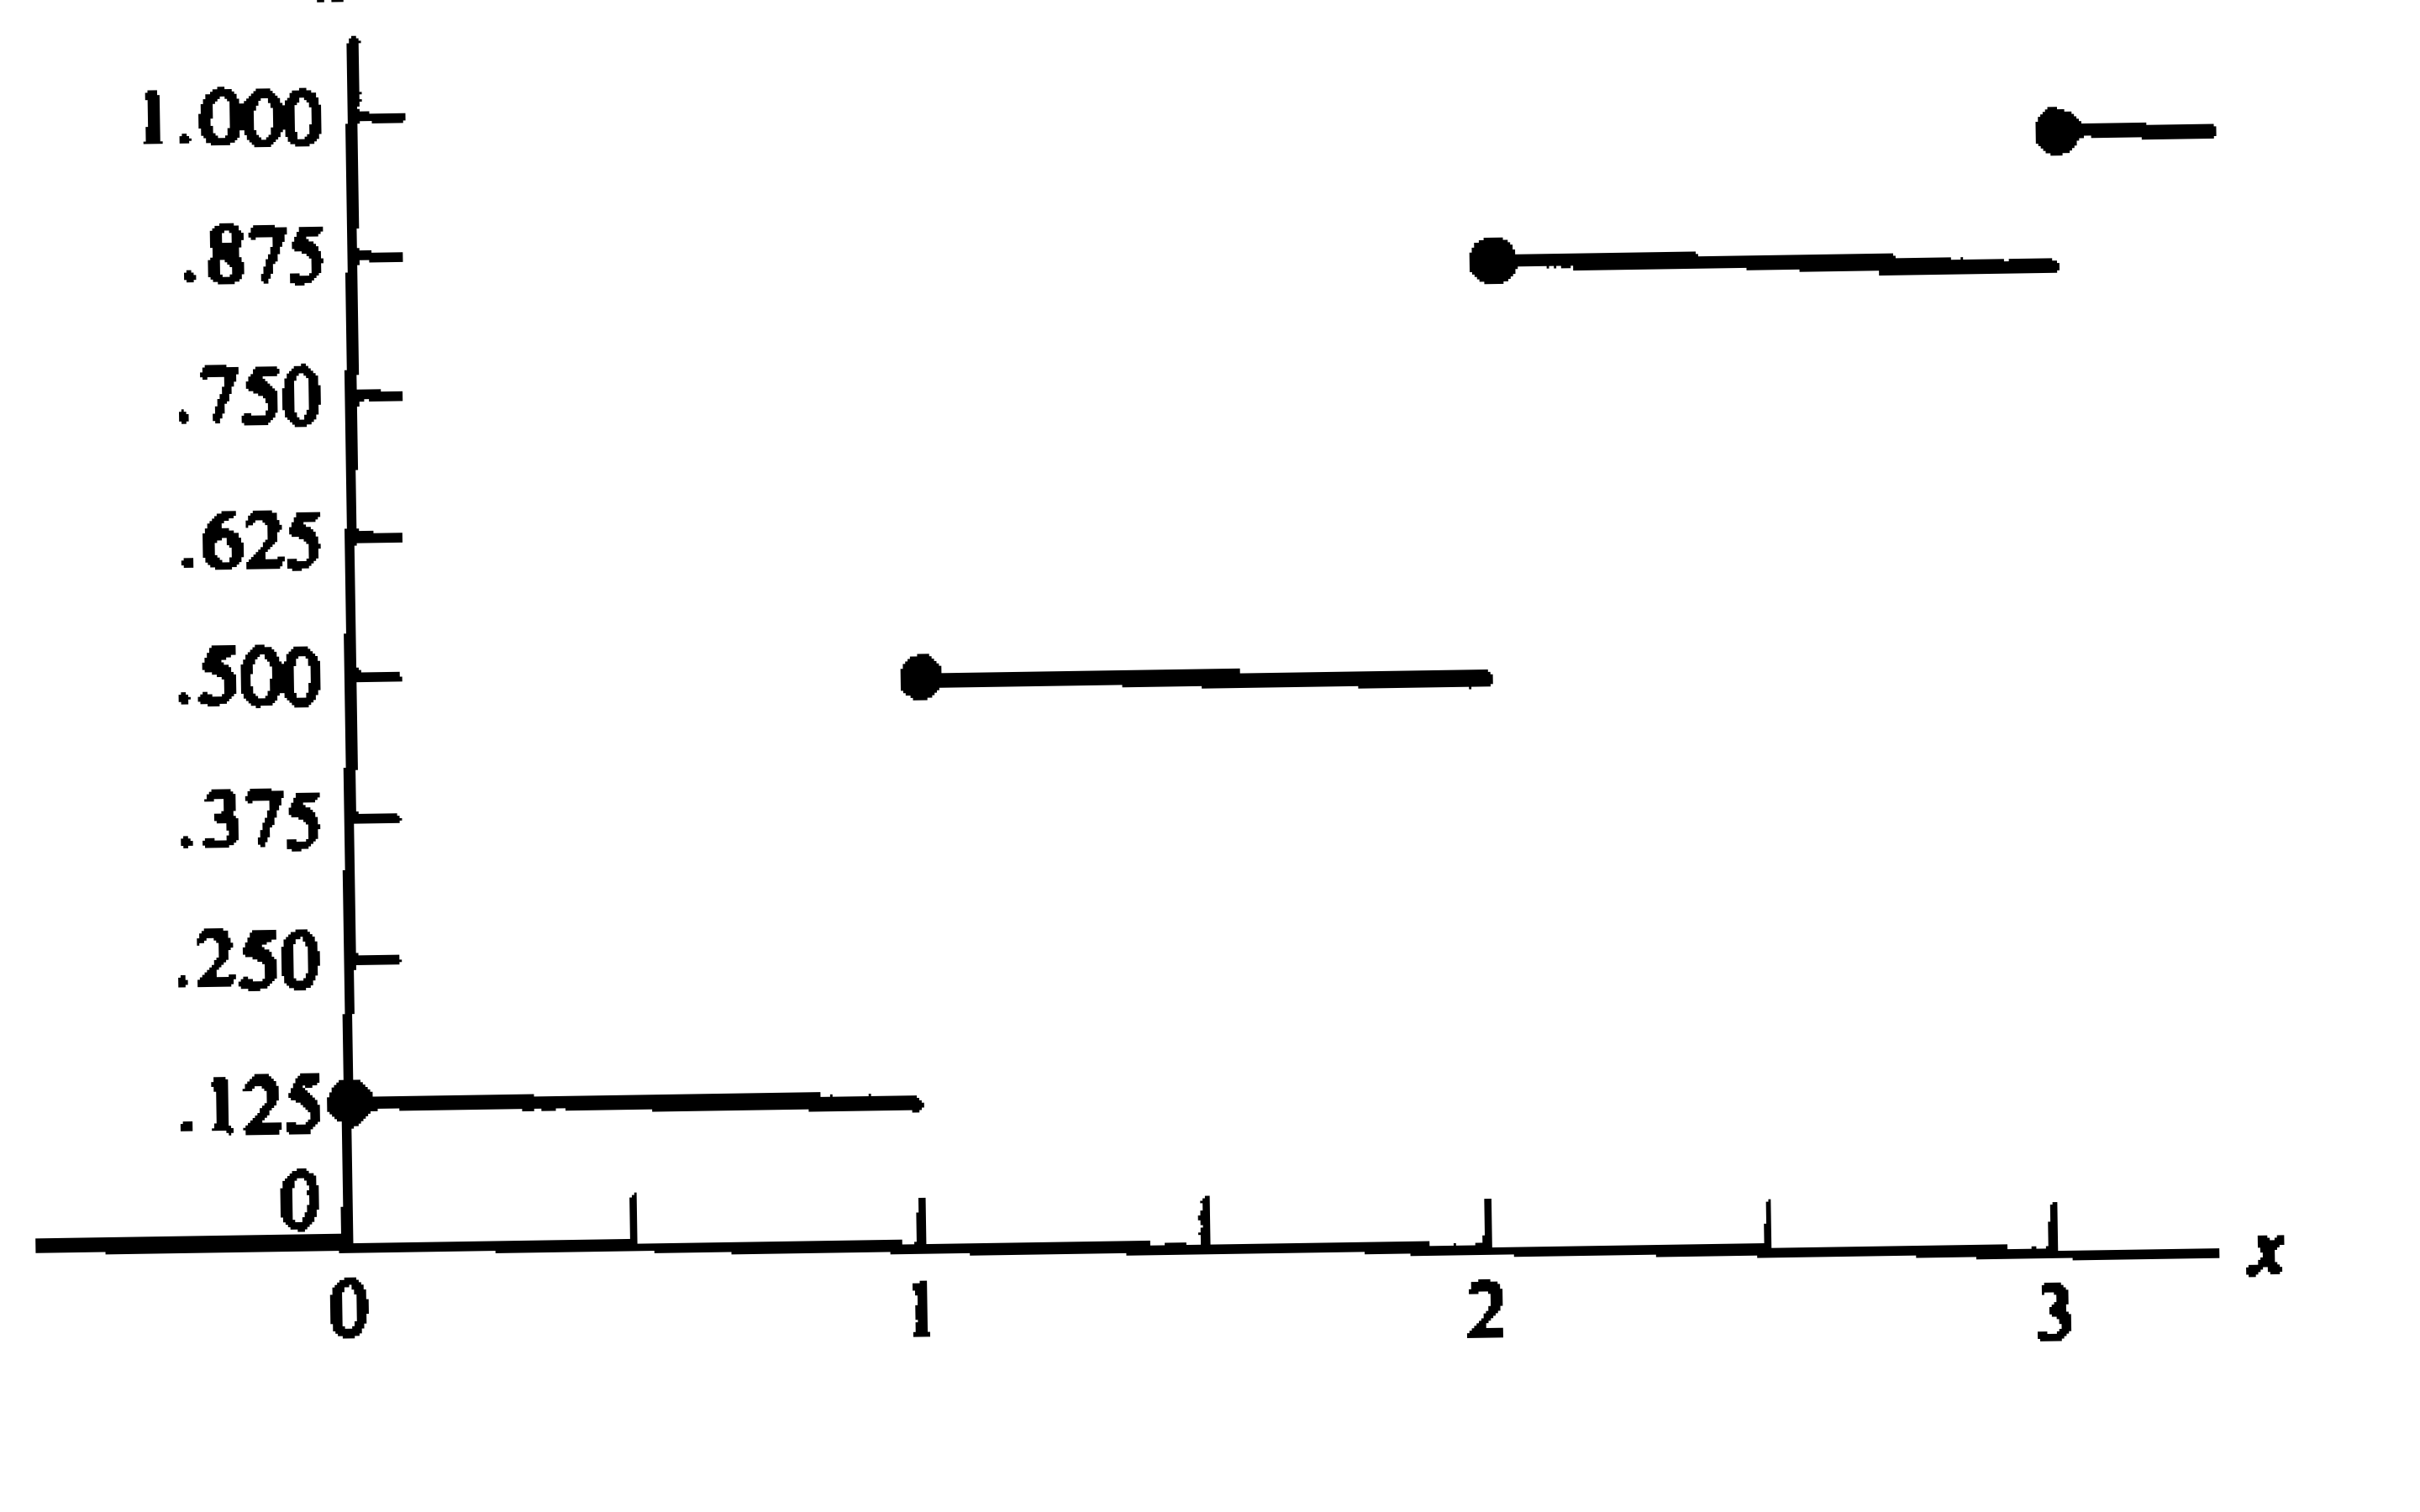
\includegraphics[scale=.25]{/Users/subhadippal/Documents/Packages/STAT230/Slides_STAT230/Unit6_STAT230_1/figs/CDF_three_coin_toss.png}
\end{center}
\begin{enumerate}
\item What is the probability that $X=2$?
\item What is the probability that $X=1.5$
\item  Obtain $P(1<X\leq 3)$
\item  Obtain $P(1\leq X< 3)$
\end{enumerate}
}\\


  \qBrd[6.9in]{airforceblue!30}{
\item 
Suppose a random variable $X$ has the following support $\support[X]= \{1, 2,3, 4, 5\}$. 
\begin{center}
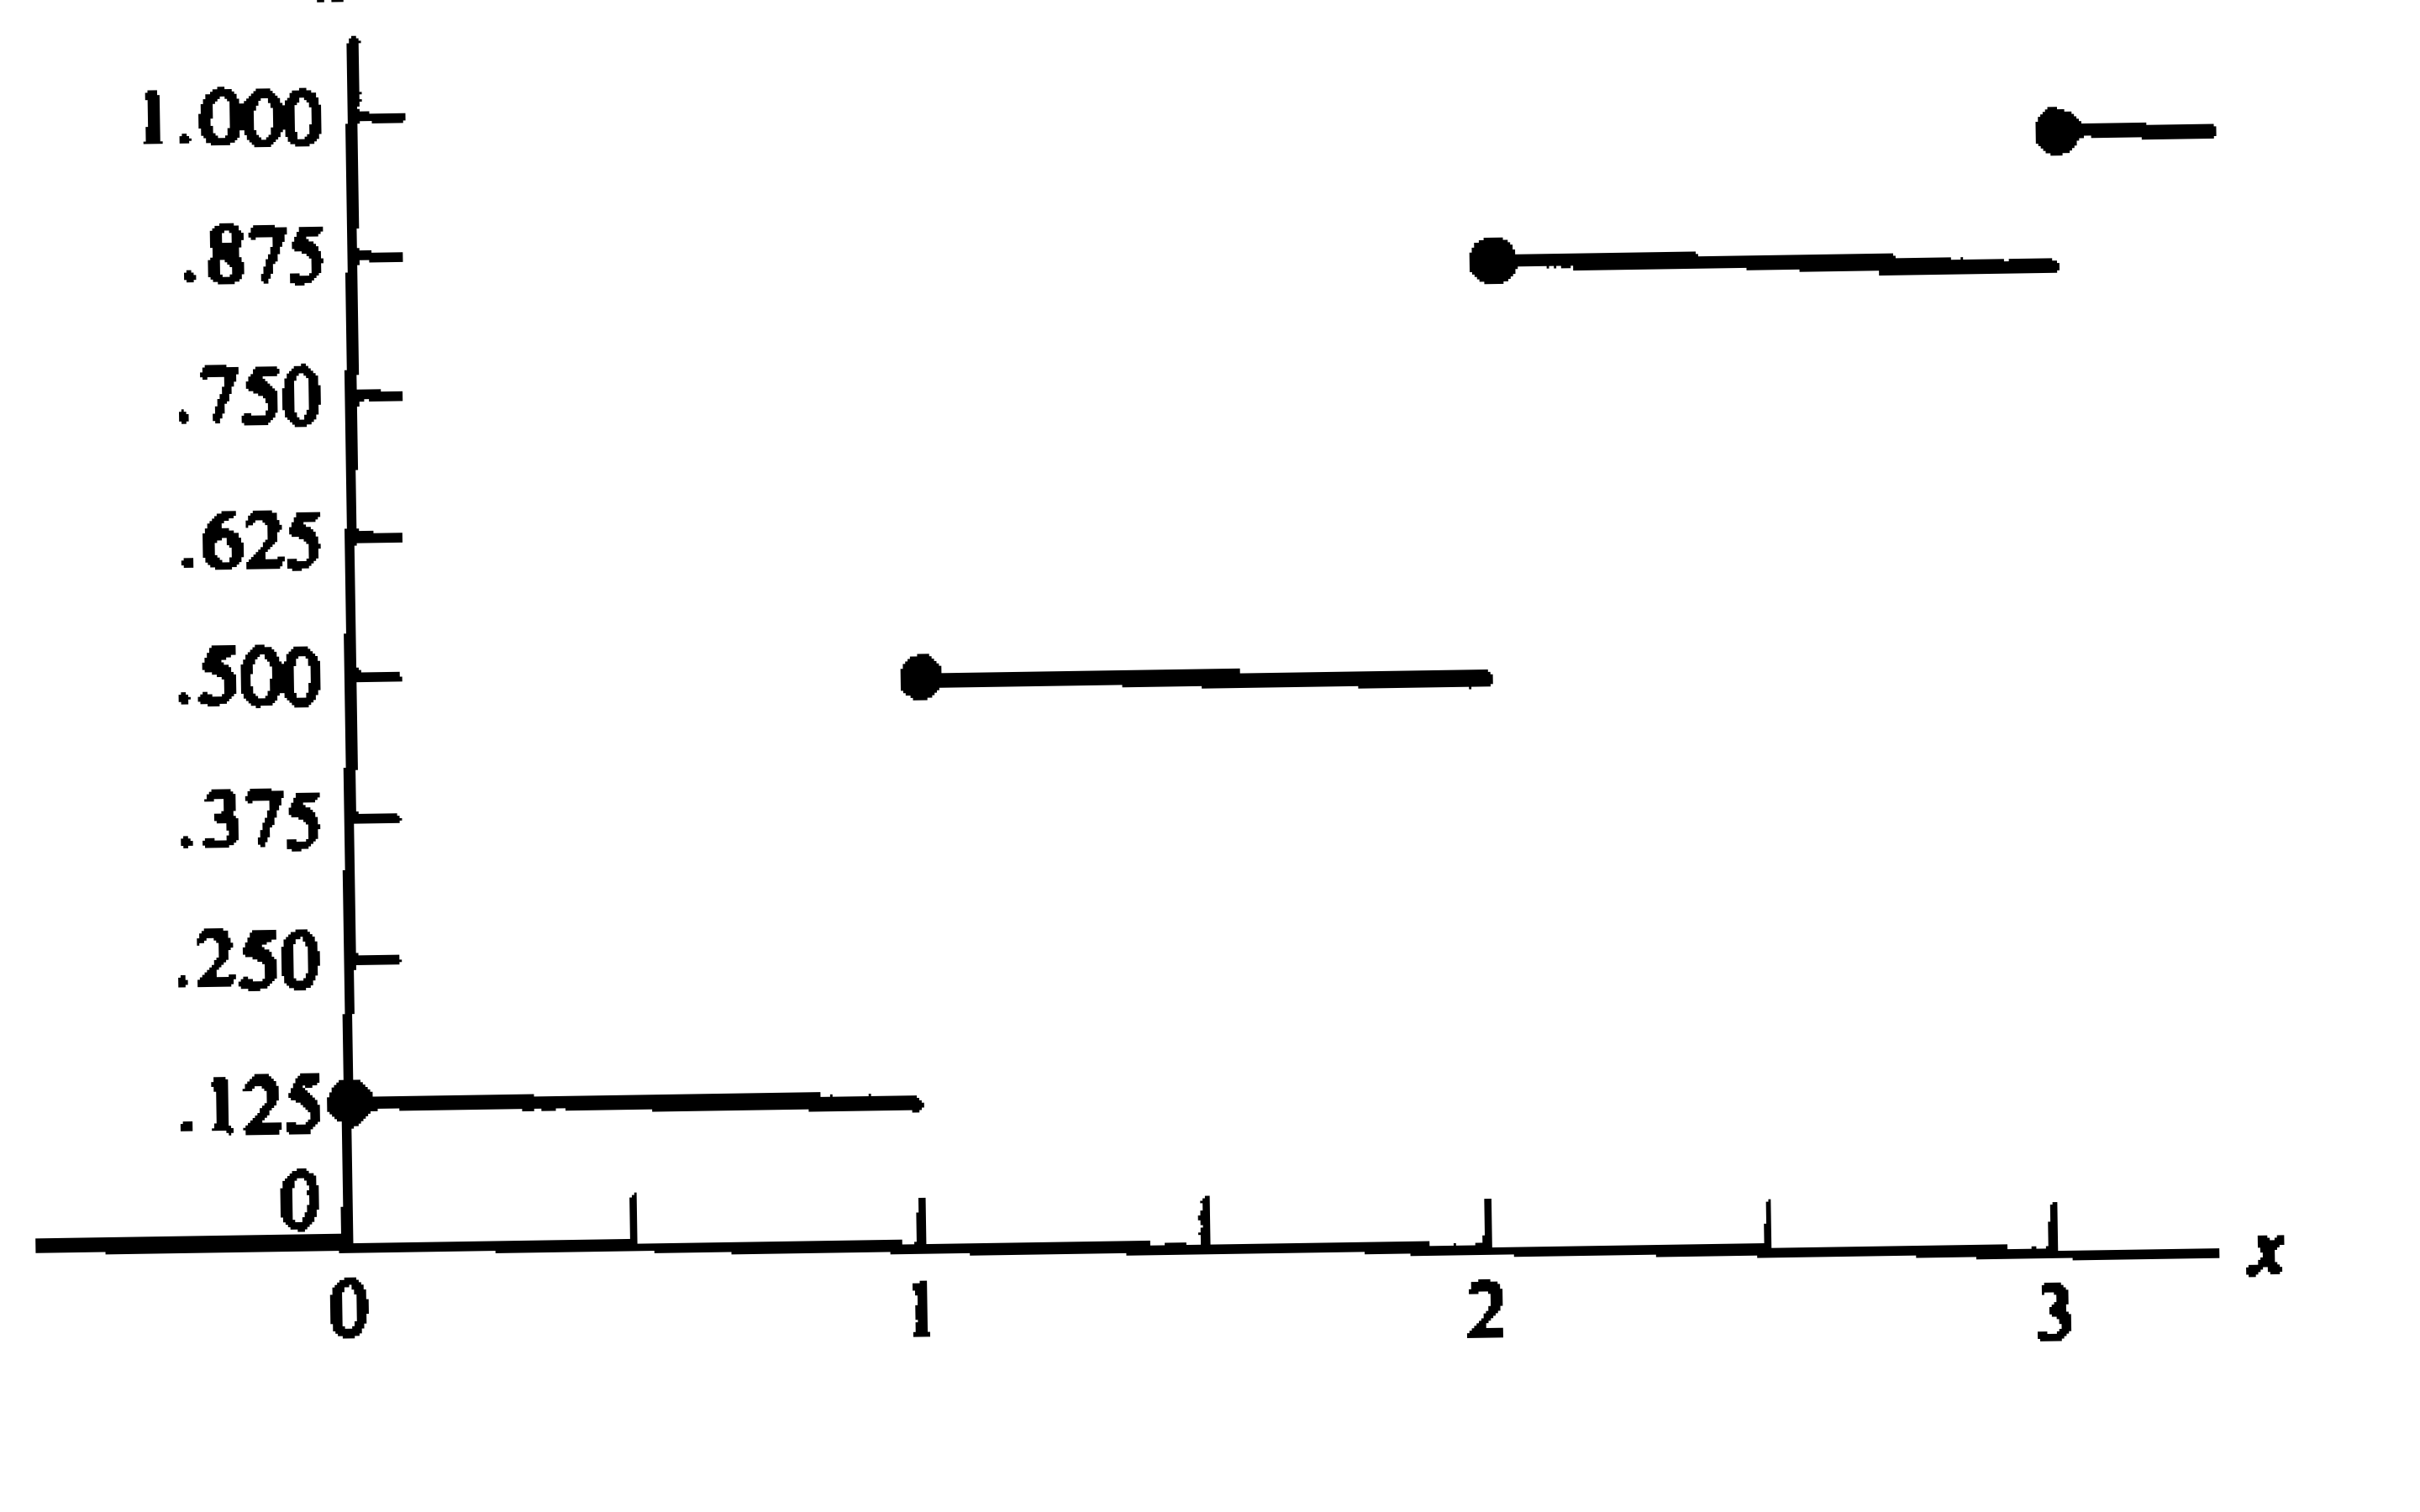
\includegraphics[scale=.25]{/Users/subhadippal/Documents/Packages/STAT230/Slides_STAT230/Unit6_STAT230_1/figs/CDF_three_coin_toss.png}
\end{center}
}\\







  \qBrd[6.9in]{airforceblue!30}{
\item 
Consider the following CDF of the random variable
$$ \displaystyle F_X(x):=\frac{1}{1+e^{-x}} \text{ for all } x\in \R.$$
\begin{center}
\includegraphics[scale=.5]{/Users/subhadippal/Documents/Packages/STAT230/Slides_STAT230/Unit6_STAT230_1/figs/logistic_CDF.png}
\end{center}
\
\begin{enumerate}
\item What is the probability that $X=0$?
\item What is the probability that $X=2$
\item  Obtain $P(0<X\leq 1)$
\item  Obtain $P( X< 2)$
\item Identify the nature of the random variable (Discrete/Continuous/ Mixture of Discrete and Continuous. )
\end{enumerate}
}\\



   \qBrd[6.9in]{amethyst!40}{
\item 
\Exmpl{amethyst}{}  Suppose that $X$ is a continuous random variable whose probability density function is given by
$$\HLTW{ f(x):= \begin{cases} 
\HLTEQ[babyblue!20]{ \HLTY{C}(4x-2x^2) }& \text{ if } 0 <x<2\\
0 & \text{ otherwise.} 
\end{cases}}$$
\vspace{-.1in}
\begin{enumerate}
\item For what value of \HLTY{C} the provided function is a valid probability density function?
\item Find $P(X>1)$.
\item Find $P( X\leq 1)$.
\item Obtain {\it mean}  (Expected value)  of X. 
\end{enumerate}
}\\



  \qBrd[6.9in]{amber!40}{\item 
\Exmpl{amber}{}  For a given IT technician in a support center, let X denote the percentage of time, out of a 40-hour work week, that he is directly serving customers. Suppose that X has a probability density function given by
$$\HLTW{ f(x):= \begin{cases} 
 3x^2& \text{ if } 0 <x<1\\
0 & \text{ otherwise.} 
\end{cases}}$$
\vspace{-.1in}
\begin{enumerate}
\item Find the probability that the technician will spend 20\% to 70\% of hisworkweek serving customers.
\item Obtain, $F(x)$, the CDF of X.
\item Use $F(x)$ to compute  $P(0.5<X\leq 0.8)$.
\item Obtain {\it mean}  (Expected value)  of X. 
\item find the {\it median}  and First Quartile ($Q_1$) of the distribution
\end{enumerate}
}



\qbx[6.9in]{applegreen!40}{\item 
\Exmpl{applegreen}{}  The lifetime in hours of a certain kind of radio tube is a random
variable having a probability density function given by
$$\HLTW{ f(x):= \begin{cases} 
\frac{100}{x^2}& \text{ if } x> 100\\
0 & \text{if 	$ x\leq 100$.} 
\end{cases}}$$
\begin{enumerate}
\item What is the probability a randomly selected tube in a radio set will have to be replaced within the  fist 150 hours of operation?
\item  Obtain the CDF function of the distribution
\item Obtain {\it median } lifetime of a randomly selected radio tube.
\item  Does the {\it  mean} / Expected value of the distribution exist?
\end{enumerate}
}\\


\qbx[6.9in]{airforceblue!40}{\item 
\Exmpl{applegreen}{}   Find $E(e^X)$ and the Moment Generating Function for the continuous random variable with probability density function 
$\HLTW{
$$ f(x):= \begin{cases} 
 1& \text{ if } 0 \leq x\leq 1\\
0 & \text{ otherwise.} 
\end{cases}$$}$
}\\



\qbx[6.9in]{amethyst!40}{\item 
\Exmpl{amethyst}{}  Let X denote the resistance of a randomly chosen resistor, and suppose that its pdf is given by
$$\HLTW{ f(x):= \begin{cases} 
 \frac{x}{18}& \text{ if } 8 \leq x\leq 10\\
0 & \text{ otherwise.} 
\end{cases}}$$
\begin{enumerate}
\item  Find $P(8.6< X\leq 9.8)$.
\item Find the median of the resistance of such resistors.
\item Find the mean and variance of X.
\end{enumerate}
}\\



\qbx[6.9in]{asparagus!40}{\item 
\Exmpl{asparagus}{}  The length of time required by students to complete a one-hour exam is a random variable with a density function given by
$$\HLTW{
f(x):= \begin{cases} 
cy^2+y& \text{ for }0\leq y\leq 1\\
0 & \text{ otherwise.} 
\end{cases}}$$
\begin{enumerate}
\item Find c that makes this function a valid probability density function.
\item Find the F(y) 
%\item Graph f(y) and F(y).
\item  Find the probability that a randomly selected student will finish in less than half an hour.
\item Find the time that 95\% of the students finish before it.
\item Given that a particular student needs at least 15 minutes to complete the exam, find the probability that she will require at least 30 minutes to finish.
\end{enumerate}
}\\



\qbx[6.9in]{apricot!40}{\item 
\Exmpl{apricot}{} The time (in min) for a lab assistant to prepare the equipment for a certain experiment is believed to have a uniform distribution with a = 25 and b = 35.
\begin{enumerate}
\item Write the probability density function of X.
\item What is the probability that preparation time exceeds 33 min?
\item What is the probability that preparation time is within 2 minmutes of the {\bf mean time}?
\end{enumerate}
}\\


\qbx[6.9in]{babyblue!40}{\item 
\Exmpl{babyblue}{} The failure rate for a type of electric light bulb is 0.002 per hour. Under the exponential model,
\begin{enumerate}
\item Find the probability that a randomly selected light bulb will fail in less than 1000 hours.
\item  Find the probability that a randomly selected light bulb will last 2000
hours before failing.
\item Find the mean and the variance of time until failure.
\item  Find the median time until failure.
\item Find the time where 95\% of these bulbs are expected to fail before it.
\end{enumerate}
}\\


\qbx[6.9in]{slateblue!40}{ \item 
\Exmpl{slateblue}{} A gasoline wholesale distributor has bulk storage tanks that hold fixed supplies and
are filled every Monday. Of interest to the wholesaler is the proportion of this supply
that is sold during the week. Over many weeks of observation, the distributor found
that this proportion could be modeled by a beta distribution with $\alpha = 4$ and $\beta = 2$.\\
\begin{enumerate}
\item Find the probability that the wholesaler will sell at least 90\% of her stock in a given week.
\item What is the expected percentage of sell in a randomly selected week. 
\end{enumerate}
}\\

\qbx[6.9in]{olive!40}{\item
\Exmpl{olive}{} The times of first failure of a unit of a brand of ink jet printers are approximately normally distributed with a mean of 1,500 hours and a standard deviation of 200 hours. Use the statistical calculator.
\begin{enumerate}
\item What fraction of these printers will fail before 1,000 hours?
\item What is the probability that the first failure time of a selected printer will fail be between 1,300 and 1700 hours?
\end{enumerate}
}\\

\qbx[6.9in]{amethyst!40}{\item 
\Exmpl{olive}{} The times of first failure of a unit of a brand of ink jet printers are approximately normally distributed with a mean of 1,500 hours and a standard deviation of 200 hours. Use the statistical calculator.
\begin{enumerate}
\item what should be the guarantee time for these printers if the manufacturer wants only 5\% to fail within the guarantee period.
\end{enumerate}
}\\


\qbx[6.9in]{amethyst!40}{\item 
\Exmpl{amethyst}{} The SAT and ACT college entrance exams are taken by thousands of students each year. The mathematics portions of each of these exams produce scores that are approximately normally distributed. In recent years, SAT mathematics exam scores have averaged 480 with standard deviation 100. The average and standard deviation for ACT mathematics scores are 18 and 6, respectively.
\begin{enumerate}
\item An engineering school sets 550 as the minimum SAT math score for new students. What percentage of students will score below 550 in a typical year?
\item  What score should the engineering school set as a comparable standard on the ACT math test?
\end{enumerate}
}\\



\qbx[6.9in]{teal!40}{ \item
\Exmpl{teal}{} An engineer working for a manufacturer of electronic components takes a large number of measurements of a particular dimension of components from the production line.  She finds that the distribution of dimensions is normal, with a mean of 2.340 cm and a standard deviation of 0.06 cm.
\begin{enumerate}
\item What percentage of measurements will be less than 2.45 cm?
\item What percentage of dimensions will be between 2.25 cm and 2.45 cm?
\item What value of the dimension will be exceeded by 98\% of the components?
\end{enumerate}
}\\

\qbx[6.9in]{babyblue!40}{ \item 
\Exmpl{babyblue}{} Of the Type A electrical resistors produced by a factory, 85\% have resistance greater than 41 ohms, and 3.7\% of them have resistance greater than 45 ohms. The resistances follow a normal distribution.
\begin{enumerate}
\item What percentage of these resistors have resistance greater than 44 ohms?
\end{enumerate}
}\\




\qBrd[4.5in]{babyblue!30}{
\item 
If $X\sim \text{Exponential}(\lambda=5)$,  then
\begin{enumerate}
\item Obtain the value of $E(X)$, $\text{Var}(X)$, and $ E(X^2)$
\item What is $E(3X+50)$?
\item What is Var$(3X+50)$?
\item What is the MGF of X?
\end{enumerate} 
}\\
\vspace{.1in}


\qBrd[4.5in]{slateblue!30}{
\item 
If $X\sim \text{Gamma}(\alpha= 10, \lambda=5)$,  then
\begin{enumerate}
\item Obtain the value of $E(X)$, $\text{Var}(X)$, and $ E(X^2)$
\item What is $E(3X+10)$?
\item What is Var$(3X-5)$?
\item What is the MGF of X?
\end{enumerate} 
}\\
\vspace{.1in}


\qBrd[4.5in]{babyblue!30}{
\item 
If $X\sim \text{Normal}(\mu= 100, \sigma=5)$,  then
\begin{enumerate}
\item What is $ E(X^2)$
\item Obtain $P(X\leq 110)$
\item Obtain $P(95\leq X\leq 110)$
\item What is the MGF of X?
\end{enumerate} 
}\\
\vspace{.1in}


\qbx[6.9in]{amethyst!40}{ \item 
\Exmpl{amethyst}{}  The joint pdf of X; Y is given by 
$$\HLTW{f_{_{X,Y}}(x,y)=
 \begin{cases}
\frac{x+y+1}{2} &  \text{ for }  0 < x <1,0 < y <1\\
0 &  \text{otherwise}\end{cases}}$$
\begin{enumerate}
\item Find the cumulative distribution function of $(X, Y)$ .
\item  Find the marginal density of X.
\item  Find the marginal density of Y .
\item Find the conditional probability of X given Y = 0.5.
\item  Use this to compute $P(X\leq 0.75 \mid Y=0.5)$
\end{enumerate}
}\\


\qbx[6.9in]{amber!40}{ \item 
\Exmpl{amber}{}  Let X, Y have joint cdf
$$\HLTW{F_{_{X,Y}}(x,y)=
 \begin{cases}
x^2y^3&  \text{ for }  0 < x <1,0 < y <1\\
 &  \text{otherwise}\end{cases}}$$
 \vspace{-.2in}
\begin{enumerate}
\item Find the joint density function of $(X, Y)$ .
\item  Find the marginal density of X.
\item  Find the marginal density of Y .
\item Find the conditional probability of X given Y = 0:5.
\item Use this to compute $P(X\geq 0.5 \mid Y=0.5)$
\end{enumerate}
}\\



\qbx[6.9in]{babyblue!40}{\item 
\Exmpl{babyblue}{}  The joint density of X and Y is given by 
$$\HLTW{f_{_{X,Y}}(x,y)=
 \begin{cases}
2e^{-x-2y}&  \text{ for }  0 < x <\infty,0 < y <\infty\\
 &  \text{otherwise}\end{cases}}$$
\begin{enumerate}
\item  Find the marginal density of X.
\item  Find the marginal density of Y .
\item Find $P(X > 1,  Y < 1) $
\item Find $P(X <Y) $
\item Find $P(X <4) $
\item  Find the conditional probability of X given Y = 1.
\item  Find the marginal density of Y .
\item Use this to compute $P(X\leq 2 \mid Y=1)$
\end{enumerate}
}\\


\qbx[6.9in]{slateblue!40}{ \item 
\Exmpl{slateblue}{}  The joint pdf of X; Y is given by 
$$\HLTW{\HLTW{f_{_{X,Y}}(x,y)=
 \begin{cases}
\frac{x+y+1}{2} &  \text{ for }  0 < x <1,0 < y <1\\
0 &  \text{otherwise}\end{cases}}}$$
\begin{enumerate}
\item Are X and Y statistically independent?
\end{enumerate}
}\\


\qbx[6.9in]{amber!40}{\item 
\Exmpl{amber}{}  Let X, Y have joint cdf
$$\HLTW{ F_{_{X,Y}}(x,y)=
 \begin{cases}
x^2y^3&  \text{ for }  0 < x <1,0 < y <1\\
 &  \text{otherwise}\end{cases}}$$
\begin{enumerate}
\item Are X and Y independent?
\end{enumerate}
}\\


\qbx[6.9in]{babyblue!40}{ \item
\Exmpl{babyblue}{}  The joint density of X and Y is given by 
$$\HLTW{f_{_{X,Y}}(x,y)=
 \begin{cases}
2e^{-x-2y}&  \text{ for }  0 < x <\infty,0 < y <\infty\\
 &  \text{otherwise}\end{cases}}$$
\begin{enumerate}
\item Are X and Y independent?
\end{enumerate}
}\\


\qbx[4.5in]{olive!40}{\item 
\Exmpl{olive}{}  Let X, Y have joint cdf
$$ \HLTW{ f_{_{X,Y}}(x,y)=
 \begin{cases}
\frac{2}{7}(x+2y)&  \text{ for }  0 < x <1,1 < y <2\\
 &  \text{otherwise}\end{cases}}$$
\begin{enumerate}
\item Find the expected value of $\frac{X}{Y^3}$
\item Find the expected value of $XY$
\end{enumerate}
}\\





\qbx[6.9in]{airforceblue!40}{\item 
\Exmpl{airforceblue}{}  Let X and Y have joint density
$$\HLTW{f_{_{X,Y}}(x,y)=
 \begin{cases}
2&  \text{ for }  x>0, y>0, x+y<1\\
 &  \text{otherwise}\end{cases}}$$
\begin{enumerate}
\item Find the covariance of X and Y .
\item Are the random variables X,  and Y statistically independent?
\end{enumerate}
}\\




\qbx[6.9in]{olive!30}{\item
\Exmpl{olive}{}  Given here is the joint probability function associated with data obtained in a study of automobile
accidents in which a child (under age 5 years) was in the car and at least one fatality occurred. Specifically, the study focused on whether or not the child survived and what type of seatbelt (if any) he or she used. Define
\begin{center}
$$\HLTW{Y_1= 
 \begin{cases}
0&  \text{ if the child survived }\\
 1&  \text{if not,}\end{cases} \text{ and,  }  
 Y_2= 
 \begin{cases}
0&  \text{ if no belt used, }\\
 1&  \text{ if adult belt used}\\
 2&  \text{ if car-seat belt used}
 \end{cases} }$$
 Notice that $Y_1$ is the number of fatalities per child and, since children's car seats usually utilize two belts, $Y_2$ is the number of seatbelts in use at the time of the accident	\\
\begin{tabular}{ |c|| c| c| } 
\toprule
\diagbox{$y_2$}{$y_1$} & \makecell{ 0}& \makecell{1}   \\ \hline
0 & 0.38&  0.17 \\\hline
1 &  0.14  & 0.02 \\\hline
2&0.24  &0.05 \\\hline
\bottomrule
\end{tabular}
\begin{enumerate}
\item What is the Marginal distribution of $Y_1$?
\item What is the Marginal distribution of $Y_2$?
\item Obtain Covariance between $Y_1$ and $Y_2$.
\end{enumerate}
\end{center}
 % Ans: 5/128
% \vspace{-.1in}
}\\



\qbx[6.9in]{babyblue!40}{\item
\Exmpl{babyblue}{}  Gasoline is to be stocked in a bulk tank once at the beginning of each week and then sold to individual customers. Let $Y_1$ denote the proportion of the capacity of the bulk
tank that is available after the tank is stocked at the beginning of the week. Because of the limited supplies, $Y_1$ varies from week to week. Let $Y_2$ denote the proportion of the capacity of the bulk tank that is sold during the week. Because $Y_1$ and $Y_2$ are both proportions, both variables take on values between 0 and 1. Further, the amount sold, $Y_2$, cannot exceed the amount available, $Y_1$.  Suppose that the joint density function for $Y_1$ and $Y_2$ is given by
$$\HLTW{f_{_{Y_1,Y_2}}(y_1,y_2)=
 \begin{cases}
3y_1&  \text{ for }  0 < x <\infty,0 \leq  y_2\leq y_1 \leq 1\\
 &  \text{otherwise}\end{cases}}$$
 \begin{enumerate}
 \item  Find the probability that less than one-half of the tank will be stocked and more than one-quarter of the tank will be sold. i.e. $P(0\leq  Y_1 \leq 0.5, Y_2 > 0.25).$
 \item What is the probability that  less than one-half of the tank will be stocked given that more than one-quarter of the tank will be sold.  
 $P(0\leq  Y_1 \leq 0.5\mid Y_2 > 0.25).$
 \item Find the marginal density of $Y_1$
 \item Find the marginal density of $Y_2$
 \item Find $E(Y_2)$
 \item Find the conditional density of $Y_2$ given $Y_1=0.25$.
 \end{enumerate}
 % Ans: 5/128
}\\




\qbx[6.9in]{airforceblue!40}{\item
\Exmpl{airforceblue}{}  The management at a fast-food outlet is interested in the joint behavior of the random variables $Y_1$, defined as the total time between a customer's arrival at the store and departure from the service window, and $Y_2$, the time a customer waits in line before reaching the service window.
Because $Y_1$ includes the time a customer waits in line, we must have $Y_1 \geq  Y_2$.  The relative frequency distribution of observed values of $Y_1$ and $Y_2$ can be modeled by the probability density function
$$\HLTW{f_{_{Y_1,Y_2}}(y_1,y_2)=
 \begin{cases}
e^{-y_1}&  \text{ for }  0 \leq  y_2\leq y_1 \leq \infty\\
 0&  \text{otherwise}\end{cases}},$$ 
 with time measured in minutes. Find
 % Ans: 5/128
% \vspace{-.1in}
 \begin{enumerate}
 \item Find Marginal Density of $Y_1$.
  \item Find Marginal Density of $Y_2$.
 \item $P(Y_1<2, Y_2>1).$
 \item $P(Y_1 \geq  2Y_2).$
 \item $P(Y_1-Y_2 \geq  1).$
 \item Find $E(Y_1-Y_2)$, expected service time. 
    \item Find Conditional  Density of $Y_2$ given $Y_1=2$.
    \item Find $E(Y_2\mid Y_1=2)$
 \end{enumerate}
}\\




\qbx[6.9in]{olive!40}{\item
\Exmpl{olive}{}Let X and Y have joint distribution.  For X and Y defined in the previous two examples,  Let $Z_1= 2X+4Y$ and $Z_2= X-2Y$
\begin{enumerate}
\item Find  $E(Z_1)$, $E(Z_2)$
\item Find Var$(Z_1)$, Var$(Z_2)$
\item Find Cov$(Z_1,Z_2)$.
\end{enumerate}
}\\

\qbx[6.9in]{teal!40}{\item 
\Exmpl{teal!60}{} \; Let X and Y be two statistically independent random variables with means $2$,  $3$ respectively. , The variances of $X,Y$ is provided as $4$ and  $2$. Let $ \HLTW{Z_1=X + 2Y + 3}$ and $\HLTW{Z_2=3X - Y}$.  Find: 
\begin{enumerate}
\item Find  $E(Z_1)$, $E(Z_2)$
\item Find Var$(Z_1)$, Var$(Z_2)$
\item Find Cov$(Z_1,Z_2)$.
\end{enumerate}
}\\

\qbx[6.9in]{babyblue!40}{\item 
Identify the Distributions along with parameters for the following moment generating functions. 
\begin{enumerate}
\item  $M_{X}(t)= (0.7+0.3e^t)^{10}$
\item $M_{X}(t)= \exp{\left(t^2\right)}$
\end{enumerate}
}\\

\qbx[6.9in]{babyblue!40}{\item 
Identify the Distributions along with parameters for the following moment generating functions. 
\begin{enumerate}
\item $M_{X}(t)=\frac{1}{\left(1-\frac{t}{5}\right)^{0.5}}$
\item $M_{X}(t)= e^{5e^t-5}$
\end{enumerate}
}\\


\qbx[6.9in]{babyblue!40}{\item 
Identify the Distributions along with parameters for the following moment generating functions. 
\begin{enumerate}
\item $M_{X}(t)= \frac{0.2e^t}{1- 0.8e^t}$
\item $M_{X}(t)=\frac{1}{\left(1-\frac{t}{10}\right)}$
\item $M_{X}(t)= \exp{\left(-2+5t^2\right)}$
\end{enumerate}
}\\


\qbx[6.9in]{teal!40}{\item 
A soft-drink machine has a random amount $Y_2$ in supply at the beginning of a given dayand dispenses a random amount $Y_1$ during the day (with measurements in gallons).  It is not resupplied during the day, and hence $Y_1\leq  Y_2$.  It has been observed that $Y_1$ and $Y_2$ have a joint density given by
$$\HLTW{   f(y_1, y_2):= \begin{cases}  
\frac{1}{2}  & 0 \leq y_1 \leq y_2 \leq 2 \\
0 & \text{ otherwise.}
   \end{cases} } $$
\begin{enumerate}
\item  Show that the marginal distribution of $Y_2$ is given as 
$$\HLTW{ f_{{{_y}_2}}(y_{_2}):= \begin{cases}
\frac{y_{_2}}{2} & 0 \leq y_{_2}\leq 2\\
0 &   \text{ otherwise.}
\end{cases} } $$
\item Obtain the conditional density of $Y_1$ given $Y_2= \frac{3}{2}$.
\item  $P(Y_1\leq \frac{1}{2} \mid Y_2= \frac{3}{2} )$
\item  $P(Y_1\leq \frac{1}{2} \mid Y_2\leq  \frac{3}{2} )$
\end{enumerate}
}\\

%
%\qbx[6.9in]{airforceblue!40}{\item 
%Ask about independence from support of the random variables
%\begin{enumerate}
%\item  
%\end{enumerate}
%}\\

%
%\qbx[6.9in]{babyblue!40}{\item 
%Misc Questions 
%\begin{enumerate}
%\item  
%\end{enumerate}
%}\\
%
%
%\qbx[6.9in]{babyblue!40}{\item 
%Misc Questions cost function of gamma random variables 
%\begin{enumerate}
%\item  
%\end{enumerate}
%}\\

\end{enumerate}




\end{document}